\section{Задача K. Робот}

\begin{frame}[t]{Задача K. Робот}

  \begin{center}
    \LARGE Задача K. Робот
  \end{center}
  \begin{center}
	  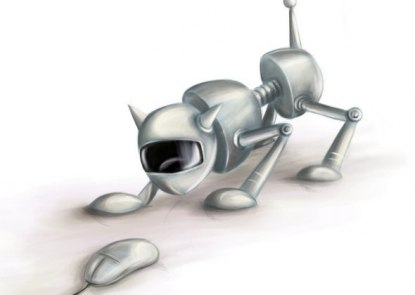
\includegraphics[width=7cm]{pics/robot.jpg}
  \end{center}
\end{frame}

\begin{frame}[t]{}
  \vspace{3cm}
  \begin{itemize}
    \item Идея задачи --- Евгений Замятин
    \item Подготовка тестов --- Евгений Замятин
    \item Разбор задачи --- Евгений Замятин
  \end{itemize}
\end{frame}

\subsection{Постановка задачи}

\begin{frame}[t]{Постановка задачи}
Входные данные:
\begin{itemize}
    \item Дано поле $n \times n$. В одной из клеток находится робот. Некоторые клетки выколоты.
    \item Дана строка $s$, состоящая из символов <<\texttt{U}>>, <<\texttt{D}>>, 
    <<\texttt{L}>>, <<\texttt{R}>>~--- программа робота.
    \item Требуется посчитать количество подстрок, 
    исполнив которые, робот не пройдет по выколотой клетке и не упрётся в границу поля.
\end{itemize}
\end{frame}

\subsection{Решение задачи}

\begin{frame}[t]{Медленное решение задачи}
\begin{itemize}
    \item Пусть робот изначально находится в клетке $(X, Y)$.
    \item Будем решать задачу отдельно для каждой выколотой клетки $(x, y)$: ближайшее вхождение выколотой клетки на суффиксе с позиции $i$.
\end{itemize}
\end{frame}

\begin{frame}[t]{Ускорение решения задачи}
\begin{itemize}
    \item Предподсчитаем массивы смещений, то есть
    массив $dx_i$~--- смещение робота от стартовой позиции после выполнения $i$ команд по оси $X$
    и аналогичный массив $dy_i$.
    \item Посмотрим на суффикс команды с позиции $i$, тогда нужно найти минимальное $t \geq i$, такое что $(X + dx_t - dx_i, Y + dy_t - dy_i) = (x, y)$.
    \item Это равносильно нахождению $t \geq i$, такое что $(X + dx_t, Y + dy_t) = (x + dx_i, y + dy_i)$.
\end{itemize}
\end{frame}

\begin{frame}[t]{Ускорение решения задачи}
\begin{itemize}
    \item Отсортируем массив смещений.
    \item Тогда для фиксированной выколотой клетки и каждого суффикса с позиции $i$ мы можем найти соответствующее $t$ методом двумя указателей по отсортированному  массиву смещений.
    \item Границы поля следует обрабатывать отдельно аналогичным образом только по фиксированной координате.
    \item Время работы: $O(t\log t + (4 + m) \cdot t)$, где $m$~--- количество выколотых клеток.
\end{itemize}
\end{frame}

